\section{Задача 2.18}
\subsection{Задание:}
Построить графический образ зависимости $ \operatorname{Rg} A = f(x) $, где
\\[1em]
$
	A(x) =
	\begin{pmatrix}
		3 & 1 & 1 & 4 \\
		x & 4 & 10 & 1 \\
		1 & 7 & 17 & 3 \\
		2 & 2 & 4 & 1
	\end{pmatrix}
$
\subsection{Решение:}
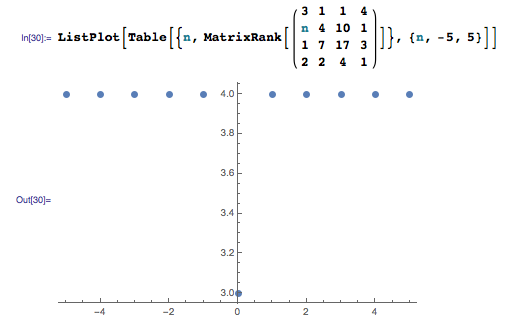
\includegraphics[scale=0.6]{task/2_18/screen.png}
\\
Видно что ранг достигает значения $ 4 $, так как в $ A $ только $ 4 $ столбца и строки, $ \max \operatorname{Rg} A = 4 $.
